\subsection{Higher Order Singular Value Decomposition}

% Was ist ein Tensor?
\begin{frame}
\frametitle{Higher Order Singular Value Decomposition}
\pause



\begin{framed}
\textbf{Definition} Tensor \\
Ein Tensor ist eine multidimensionale Matrix $\pmb{\mathcal{X}}  \in \mathbb{R}^{I_1 \times I_2 \times \dots \times I_N}$.
Die Ordnung ist die Anzahl der Dimensionen, in diesem Fall $N$. 
\end{framed}

\begin{figure}[ht]
	\centering
  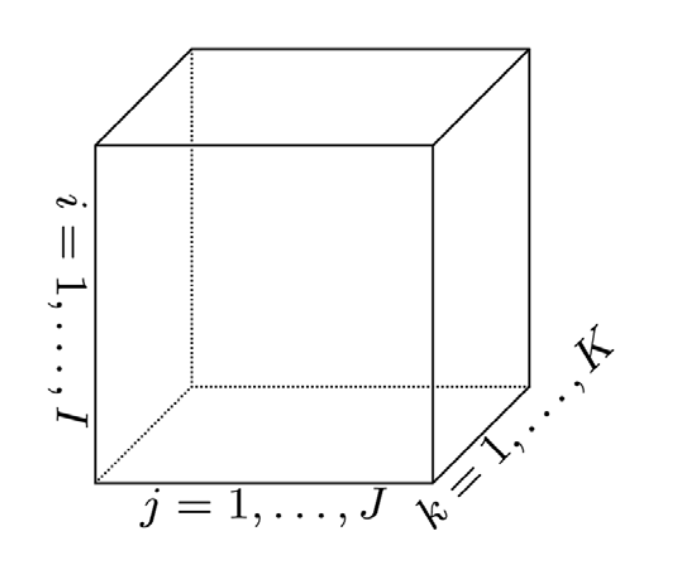
\includegraphics[width=0.4\textwidth]{tensorOrdnung3.png}
	\caption{Tensor dritter Ordnung $\pmb{\mathcal{X}}  \in \mathbb{R}^{I \times J \times K}$ \cite[456]{Kolda}}
	\label{fig:tensorOrdnung3}
\end{figure}

\end{frame}


% Tensor Definition und Eigenschaften
\begin{frame}
\frametitle{Tensoren: Definitionen und Eigenschaften}

\begin{framed}
\textbf{Bemerkung} Tensor-Charakteristiken \\
Es sei $\pmb{\mathcal{X}}  \in \mathbb{R}^{I_1 \times I_2 \times \dots \times I_N}$ ein Tensor.
\begin{itemize}
\item[a)] Den Tensor $\pmb{\mathcal{X}}$ nennt man kubisch genau dann, wenn $I_i = I_j$ für alle $i,j$.
\item[b)] Einen kubischen Tensor nennt man supersymmetrisch genau dann, wenn die Elemente des Tensors konstant bleiben unter jeglicher Permutation der Indizes.
\item[c)] Einen Tensor nennt man stückweise symmetrisch, wenn die Elemente konstant bleiben unter der Permutation von mindestens zwei Indizes.
\end{itemize}

\end{framed}

\end{frame}

\begin{frame}

\begin{framed}
\textbf{Definition} Diagonal \\
Den Tensor $\pmb{\mathcal{X}}$ nennt man diagonal, wenn
$\, x_{ \, i_1 \,, \, \dots \, , \, i_N \, } \, \neq 0$ genau dann wenn \\ $\, i_1 = \dots = i_N$.
\end{framed}

\pause

\begin{framed}
\textbf{Definition} Faser \\
Eine Faser ist das multidimensionale Analog zu Matrixspalten und Matrixzeilen. Wir definieren eine Faser, indem wir jeden Index abgesehen von einem festhalten.

\end{framed}

\end{frame}


% Tensor Entfaltung
\begin{frame}
\frametitle{Tensor-Entfaltung}
\textbf{Wir wollen unseren Tensor als Matrix darstellen.} \\
\pause
\begin{itemize}
\item $Mode-n$ Entfaltung von $\pmb{\mathcal{X}}$ wird mit $\bold{X}_{(n)}$ notiert.
\item Ordnet die $mode-n$ Fasern in die Spalten der Ergebnismatrix.
\item Formal ist es eine Abbildung des Indize N-tupels $(i_1,\dots,i_N)$ auf das Matrixindize-Tupel $(i_n,j) $
\begin{equation*}
j=1+\sum_{\substack{k=1 \\ k \neq n}}^{N} (i_k-1)J_k \text{ mit } J_k = \prod_{\substack{m=1 \\ m \neq n}}^{k-1} I_m \, .
\end{equation*}
\end{itemize}


\end{frame}


% n-mode Produkt
\begin{frame}
\frametitle{Tensor-Matrix Produkt}
\begin{framed}

\textbf{Definition} $n-mode$ Produkt \\
Das n-mode Produkt des Tensors $\pmb{\mathcal{X}}$ mit einer Matrix $\bold{U} \in \mathbb{R}^{J \times I_n}$ wird mit $\pmb{\mathcal{X}} \times_n \bold{U}$ notiert. Die Ergebnismatrix hat die Größe $I_1 \times \dots I_{n-1} \times J \times I_{n+1} \times \dots I_N$
\begin{equation*}
	(\, \pmb{\mathcal{X}} \times_n \bold{U} \, )_{\, i_1 \, \dots \, i_{n-1} \, j \, i_{n+1}\, \dots \, i_N} = \sum_{i_n = 1}^{I_n} x_{\, i_1 \, \dots \, i_N} \, u_{j \, i_n}
\end{equation*}


\end{framed}

\pause

Jedes $n-mode$ Produkt kann mit Hilfe von entfalteten Tensoren äquivalent ausgedrückt werden.
\begin{equation*}
\pmb{\mathcal{Y}} = \pmb{\mathcal{X}} \times_n \bold{U} \Longleftrightarrow \bold{Y}_{(n)} = \bold{U} \bold{X}_{(n)}
\end{equation*}

\end{frame}

% HOSVD
\begin{frame}
\frametitle{Higher Order Singular Value Decomposition}
\textbf{Ziel } Sinnvolle Zerlegung eines Tensors. \\

\begin{itemize}
\item Für Matrizen gibt es die Singulärwertzerlegung. $\, ( M=U \Sigma V^T ) $  
\item Für Tensoren haben wir die Higher Order Value Decomposition (HOSVD) oder auch Tucker Decomposition genannt.
\item Die HOSVD ist eine multidimensionale Hauptkomponentenanalyse.
\item Zerlegt Tensor in einen Kerntensor (Core Tensor), welcher das pendant zum $\Sigma$ ist und mehreren orthogonalen Matrizen.
\end{itemize}

\end{frame}

% HOSVD Formal
\begin{frame}
\frametitle{Higher Order Singular Value Decomposition}
Allgemein ist die HOSVD des Tensors $\pmb{\mathcal{X}}  \in \mathbb{R}^{I_1 \times I_2 \times \dots \times I_N}$ gegeben durch
\begin{equation*}
\pmb{\mathcal{X}}= \pmb{\mathcal{G}} \times_1 \, A^{(1)} \, \dots \, \times_N A^{(N)} \, .
\end{equation*}
Man kann äquivalent die HOSVD, wie in  \cite[462]{Kolda}, auch mit entfalteten Tensoren wie folgt angeben
\begin{equation*} \label{eq:tensortensor}
\bold{X}_{(n)} = A^{(n)} \, \bold{G}_{(n)} \, ( \, A^{(N)} \, \otimes  \, \dots \, \otimes \, A^{(n+1)} \, \otimes A^{(n-1)} \otimes \dots \otimes \, A^{(1)} \, )^{T} \, .
\end{equation*}

\end{frame}

% HOSVD Example
\begin{frame}
\frametitle{Beispiel}
Es sei $\pmb{\mathcal{X}} \in \mathbb{R}^{I \times J \times K}$.  Dann kann man den Tensor $\pmb{\mathcal{X}}$ zerlegen in 
\begin{equation}
{\pmb{\mathcal{X}}} \approx  \pmb{\mathcal{G}}  \times_1 A \times_2 B \times_3 C  \, ,
\end{equation}

wobei $A \in \mathbb{R}^{I \times P}$, $B \in \mathbb{R}^{J \times Q}$ und $C \in \mathbb{R}^{K \times R}$ die orthogonalen Faktormatrizen sind.
Der Tensor ${\cal G}$ bezeichnet den Kerntesor und zeigt wie hoch die Korrelation zwischen den verschiedenen Komponenten ist.


\begin{figure}[ht]
	\centering
  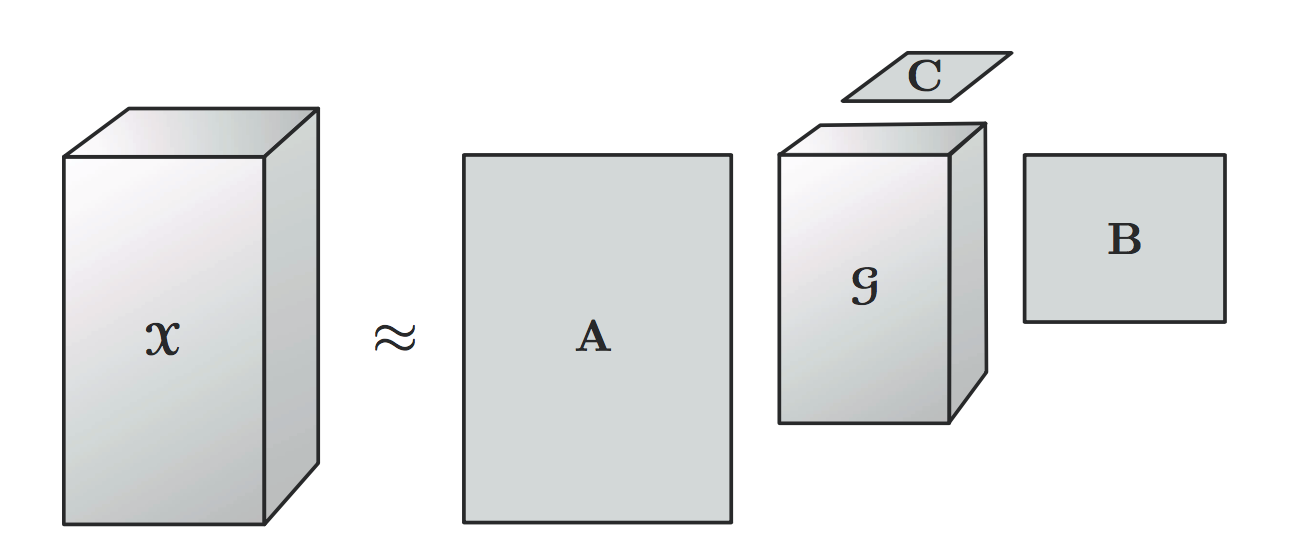
\includegraphics[width=0.6\textwidth]{hosvdTensor.png}
	\caption{HOSVD eines Tensors dritter Ordnung \cite[475]{Kolda}}
	\label{fig:hosvdTensor}
\end{figure}
\end{frame}

% Berechnung der HOSVD
\begin{frame}
\frametitle{Berechnung}
\begin{framed}
Die Berechnung der HOSVD von ${\pmb{\mathcal{X}}}  \in \mathbb{R}^{I_1 \times I_2 \times \dots \times I_N}$ funktioniert wie folgt:
\begin{enumerate}
\item Berechne die mode-k Entfaltungen $\bold{X}_{(k)}$ für alle k.
\item Berechne die Singulärwertzerlegung $\bold{X}_{(k)}=U_k \Sigma_k V_k^T$ und speichere $U_k$.
\item Der Kerntensor ${\pmb{\mathcal{G}}} $ ergibt sich aus der Projektion des Tensors auf die Tensorbasis geformt von den Faktormatrizen  $ \, \{ \, U_k \, \}_{k=1}^{N}$  also $\, \, {\pmb{\mathcal{G}}} ={\pmb{\mathcal{X}}}  \times_{n=1}^{N} \, U_n^T$.
\end{enumerate}
\end{framed}
\end{frame}


% Kronecker Produkt
\subsection{Kronecker Produkt}
\begin{frame}
\frametitle{Kronecker Produkt}

\begin{framed}
\textbf{Lemma}  (Invertieren des Kronecker Produkts) \\
Es seien $A \in \mathbb{R}^{i \times i}$ und $B \in \mathbb{R}^{j \times j}$ invertierbar, so ist auch $(A \otimes B)$ invertierbar. 
\begin{equation*}
(A \otimes B)^{-1} = A^{-1} \otimes B^{-1} \, . 
\end{equation*}
Für die Moore Penrose Pseudoinversen gilt analog
\begin{equation*}
(A \otimes B)^{+} = A^{+} \otimes B^{+} \, .
\end{equation*}
\end{framed}

\end{frame}

\begin{frame}
\begin{framed}
\textbf{Lemma} (Transponieren) \label{lemma:transpose} \\
Es seien $A,B$ beliebige Matrizen. Es gilt
\begin{equation*}
(A \otimes B)^T=A^T \otimes B^T \, .
\end{equation*}
\end{framed}

\begin{framed}
\textbf{Lemma} (Matrixprodukt und Kronecker Produkt) \\
Es seien $A,B,C,D$ Matrizen, deren Matrizenprodukte $AC$ und $BD$ definiert sind. Dann gilt
\begin{equation*}
AC \otimes BD = (A \otimes B)(C \otimes D).
\end{equation*}

\end{framed}

\end{frame}